% Standalone build of the OA-RLAIF method figure. The PDF page is sized exactly to the drawing.
% Build: pdflatex -interaction=nonstopmode oa_rlaif_pipeline.tex
\documentclass{article}
\usepackage[T1]{fontenc}
\usepackage{lmodern}
\usepackage{amsmath,amssymb}
\usepackage{tikz}
\usetikzlibrary{positioning,fit,backgrounds,arrows.meta,calc,shapes.symbols,patterns}
% Okabe-Ito colorblind-safe palette used by the OA-RLAIF figures.
\definecolor{okOrange}{HTML}{E69F00}
\definecolor{okSky}{HTML}{56B4E9}
\definecolor{okGreen}{HTML}{009E73}
\definecolor{okYellow}{HTML}{F0E442}
\definecolor{okBlue}{HTML}{0072B2}
\definecolor{okVerm}{HTML}{D55E00}
\definecolor{okPurple}{HTML}{CC79A7}
\definecolor{okGrey}{HTML}{6E6E6E}

\pagestyle{empty}
\setlength{\parindent}{0pt}\setlength{\textwidth}{50cm}\setlength{\textheight}{50cm}
\newsavebox\figbox
\begin{document}
\sbox\figbox{% OA-RLAIF method figure (TikZ body). \input this inside a figure* environment.
% Requires: tikz with libraries positioning, fit, backgrounds, arrows.meta, calc,
% shapes.symbols, patterns; amsmath, amssymb; colors defined in oa_rlaif_colors.tex.
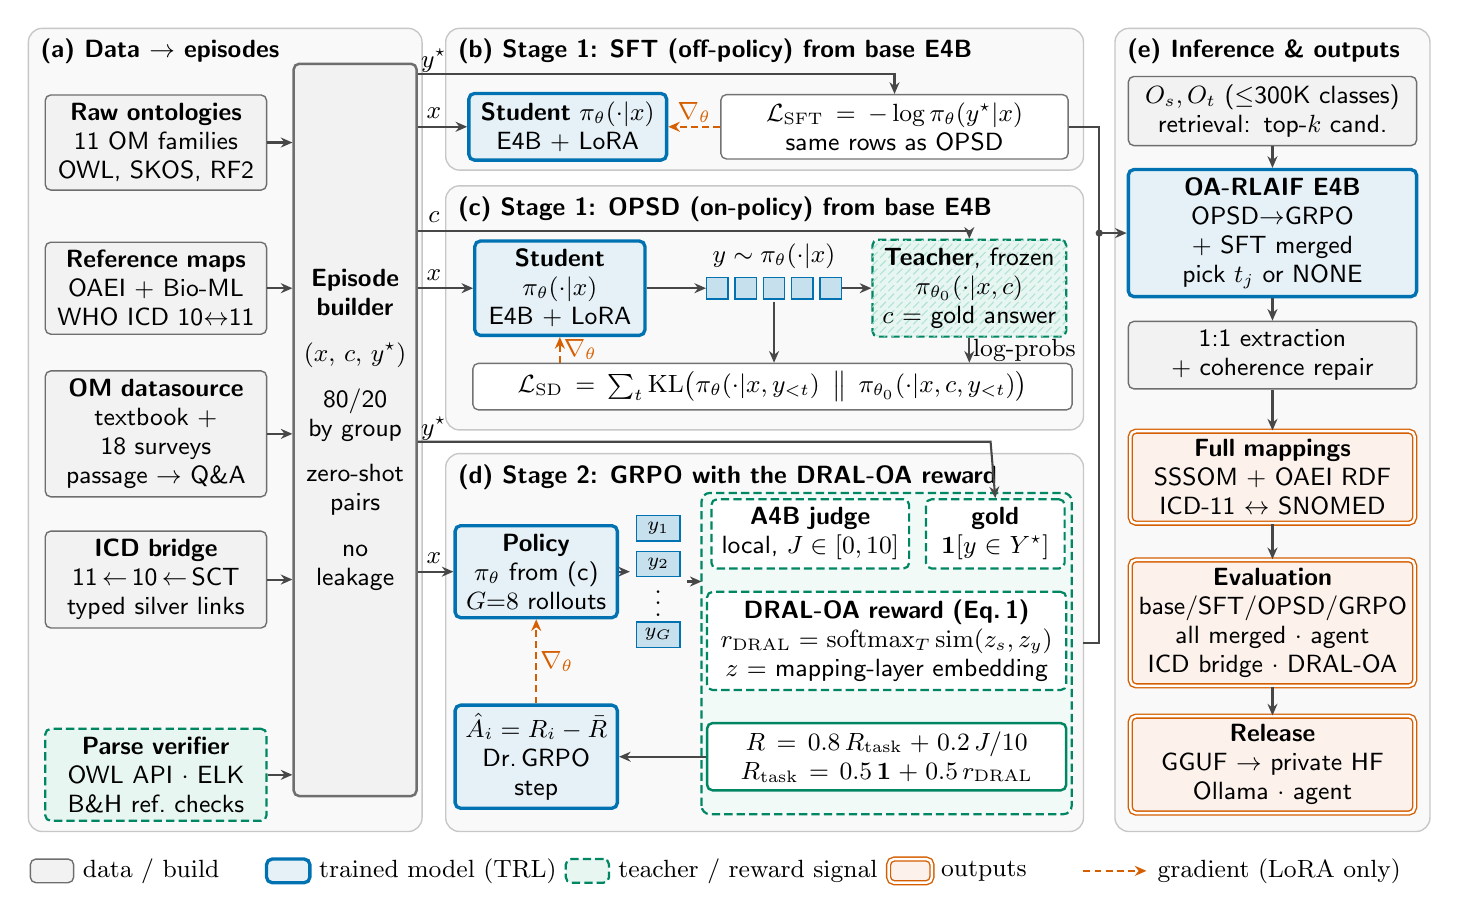
\begin{tikzpicture}[
  x=1cm, y=1cm,
  font=\fontsize{9}{10.5}\selectfont\sffamily,
  box/.style={draw, rounded corners=2pt, line width=0.5pt, align=center, inner sep=3pt},
  data/.style={box, draw=okGrey, fill=okGrey!9},
  train/.style={box, draw=okBlue, fill=okBlue!10, line width=1.2pt},
  signal/.style={box, draw=okGreen!85!black, fill=okGreen!9, dash pattern=on 3pt off 1.5pt, line width=0.8pt},
  outp/.style={box, draw=okVerm, fill=okVerm!8, double, double distance=0.9pt, line width=0.5pt},
  panel/.style={draw=black!22, fill=black!2.5, rounded corners=5pt, line width=0.5pt},
  ptitle/.style={anchor=north west, inner sep=0pt, font=\fontsize{9.5}{11}\selectfont\sffamily\bfseries},
  flow/.style={-{Stealth[length=4.2pt,width=3.6pt]}, line width=0.75pt, draw=black!72},
  grad/.style={-{Stealth[length=4.2pt,width=3.6pt]}, line width=0.9pt, draw=okVerm, dash pattern=on 2.5pt off 1.5pt},
  lab/.style={inner sep=1pt, font=\fontsize{9}{10.5}\selectfont},
  tok/.style={draw=okBlue, fill=okBlue!22, minimum width=0.27cm, minimum height=0.27cm, inner sep=0pt, line width=0.5pt},
]
\newcommand{\one}{\mathbf{1}}

% ---------------- panels ----------------
\draw[panel] (0,0) rectangle (5.0,10.2);
\draw[panel] (5.3,8.4) rectangle (13.4,10.2);
\draw[panel] (5.3,5.1) rectangle (13.4,8.2);
\draw[panel] (5.3,0) rectangle (13.4,4.8);
\draw[panel] (13.8,0) rectangle (17.8,10.2);
\node[ptitle] at (0.15,10.07) {(a) Data $\to$ episodes};
\node[ptitle] at (5.45,10.07) {(b) Stage 1: SFT (off-policy) from base E4B};
\node[ptitle] at (5.45,8.07) {(c) Stage 1: OPSD (on-policy) from base E4B};
\node[ptitle] at (5.45,4.67) {(d) Stage 2: GRPO with the DRAL-OA reward};
\node[ptitle] at (13.95,10.07) {(e) Inference \& outputs};

% ---------------- (a) data -> episodes ----------------
\node[data, text width=2.6cm] (raw) at (1.62,8.75) {\textbf{Raw ontologies}\\11 OM families\\OWL, SKOS, RF2};
\node[data, text width=2.6cm] (ref) at (1.62,6.9) {\textbf{Reference maps}\\OAEI + Bio-ML\\WHO ICD 10$\leftrightarrow$11};
\node[data, text width=2.6cm] (book) at (1.62,5.05) {\textbf{OM datasource}\\textbook + 18 surveys\\passage $\to$ Q\&A};
\node[data, text width=2.6cm] (icd) at (1.62,3.2) {\textbf{ICD bridge}\\11$\,\leftarrow\,$10$\,\leftarrow\,$SCT\\typed silver links};
\node[data, text width=1.35cm, minimum height=9.3cm, line width=0.9pt] (build) at (4.15,5.1)
  {\textbf{Episode}\\\textbf{builder}\\[6pt]$(x,\,c,\,y^\star)$\\[6pt]80/20\\by group\\[6pt]zero-shot\\pairs\\[6pt]no\\leakage};
\node[signal, text width=2.6cm] (ver) at (1.62,0.72) {\textbf{Parse verifier}\\OWL API $\cdot$ ELK\\B\&H ref.\ checks};
\foreach \s in {raw,ref,book,icd,ver} \draw[flow] (\s.east) -- (\s.east -| build.west);

% ---------------- (b) stage 1: SFT ----------------
\node[train, text width=2.3cm] (sftstu) at (6.85,8.95) {\textbf{Student} $\pi_\theta(\cdot|x)$\\E4B + LoRA};
\node[box, draw=black!55, fill=white, text width=4.2cm] (sftloss) at (11.0,8.95)
  {$\mathcal{L}_{\mathrm{SFT}}=-\log\pi_\theta(y^\star|x)$\\same rows as OPSD};
\draw[grad] (sftloss.west) -- (sftstu.east) node[lab, midway, above, text=okVerm] {$\nabla_\theta$};
\draw[flow] (build.east |- sftstu.west) -- (sftstu.west);
\node[lab] at (5.15,9.12) {$x$};
\draw[flow] (build.east |- 0,9.62) -- (11.0,9.62) -- (sftloss.north);
\node[lab] at (5.15,9.79) {$y^\star$};

% ---------------- (c) stage 1: OPSD ----------------
\node[train, text width=1.95cm] (stu) at (6.75,6.9) {\textbf{Student}\\$\pi_\theta(\cdot|x)$\\E4B + LoRA};
\foreach \i in {0,...,4} \node[tok] (t\i) at (8.75+\i*0.36,6.9) {};
\node[lab] at (9.47,7.3) {$y\sim\pi_\theta(\cdot|x)$};
\node[signal, text width=2.25cm, postaction={pattern=north east lines, pattern color=okGreen!30}] (tea) at (11.95,6.9)
  {\textbf{Teacher}, frozen\\$\pi_{\theta_0}(\cdot|x,c)$\\$c$ = gold answer};
\node[box, draw=black!55, fill=white, text width=7.4cm] (loss) at (9.45,5.65)
  {$\mathcal{L}_{\mathrm{SD}}=\sum_{t}\mathrm{KL}\big(\pi_\theta(\cdot|x,y_{<t})\;\big\|\;\pi_{\theta_0}(\cdot|x,c,y_{<t})\big)$};
\draw[flow] (stu.east) -- (t0.west);
\draw[flow] (t4.east) -- (tea.west);
\draw[flow] (9.47,6.73) -- (9.47,6.73 |- loss.north);
\draw[flow] (tea.south) -- (tea.south |- loss.north) node[lab, pos=0.5, right] {log-probs};
\draw[grad] (stu.south |- loss.north) -- (stu.south) node[lab, midway, right, text=okVerm] {$\nabla_\theta$};
\draw[flow] (build.east |- stu.west) -- (stu.west);
\node[lab] at (5.15,7.07) {$x$};
\draw[flow] (build.east |- 0,7.63) -- (11.95,7.63) -- (tea.north);
\node[lab] at (5.15,7.8) {$c$};

% ---------------- (d) stage 2: GRPO ----------------
\node[train, text width=1.85cm] (pol) at (6.45,3.3) {\textbf{Policy}\\$\pi_\theta$ from (c)\\$G{=}8$ rollouts};
\node[tok, minimum width=0.55cm, minimum height=0.32cm] (y1) at (8.0,3.85) {\scriptsize$y_1$};
\node[tok, minimum width=0.55cm, minimum height=0.32cm] (y2) at (8.0,3.4) {\scriptsize$y_2$};
\node[lab] at (8.0,3.0) {$\vdots$};
\node[tok, minimum width=0.55cm, minimum height=0.32cm] (yG) at (8.0,2.5) {\scriptsize$y_G$};
\node[fit=(y1)(yG), inner sep=2pt] (roll) {};
\draw[flow] (pol.east) -- (pol.east -| roll.west);
\draw[signal, rounded corners=3pt, fill=okGreen!5] (8.55,0.22) rectangle (13.25,4.3);
\node[signal, fill=white, text width=2.3cm] (judge) at (9.93,3.78) {\textbf{A4B judge}\\local, $J\in[0,10]$};
\node[signal, fill=white, text width=1.55cm] (gold) at (12.28,3.78) {\textbf{gold}\\$\one[y\in Y^\star]$};
\node[signal, fill=white, text width=4.35cm] (dral) at (10.9,2.42)
  {\textbf{DRAL-OA reward (Eq.\,1)}\\$r_{\mathrm{DRAL}}=\mathrm{softmax}_{T}\,\mathrm{sim}(z_s,z_y)$\\\mbox{$z$ = mapping-layer embedding}};
\node[box, draw=okGreen!85!black, fill=white, line width=0.9pt, text width=4.35cm] (rew) at (10.9,0.95)
  {$R=0.8\,R_{\mathrm{task}}+0.2\,J/10$\\$R_{\mathrm{task}}=0.5\,\one+0.5\,r_{\mathrm{DRAL}}$};
\draw[flow] (roll.east) -- (roll.east -| 8.55,0);
\node[train, text width=1.85cm] (adv) at (6.45,0.95) {$\hat A_i=R_i-\bar R$\\Dr.\,GRPO step};
\draw[flow] (rew.west) -- (adv.east);
\draw[grad] (adv.north) -- (pol.south) node[lab, midway, right, text=okVerm] {$\nabla_\theta$};
\draw[flow] (build.east |- pol.west) -- (pol.west);
\node[lab] at (5.15,3.47) {$x$};
\draw[flow] (build.east |- 0,4.95) -- (12.22,4.95) -- (gold.north);
\node[lab] at (5.15,5.12) {$y^\star$};

% ---------------- (e) inference & outputs ----------------
\node[data, text width=3.45cm] (d1) at (15.8,9.15) {$O_s,O_t$ ($\le$300K classes)\\retrieval: top-$k$ cand.};
\node[train, text width=3.45cm] (d2) at (15.8,7.6) {\textbf{OA-RLAIF E4B}\\OPSD$\to$GRPO + SFT merged\\pick $t_j$ or NONE};
\node[data, text width=3.45cm] (d3) at (15.8,6.05) {1:1 extraction\\+ coherence repair};
\node[outp, text width=3.4cm] (d4) at (15.8,4.5) {\textbf{Full mappings}\\SSSOM + OAEI RDF\\ICD-11 $\leftrightarrow$ SNOMED};
\node[outp, text width=3.4cm] (d5) at (15.8,2.65) {\textbf{Evaluation}\\base/SFT/OPSD/GRPO\\all merged $\cdot$ agent\\ICD bridge $\cdot$ DRAL-OA};
\node[outp, text width=3.4cm] (d6) at (15.8,0.85) {\textbf{Release}\\GGUF $\to$ private HF\\Ollama $\cdot$ agent};
\draw[flow] (d1) -- (d2); \draw[flow] (d2) -- (d3); \draw[flow] (d3) -- (d4);
\draw[flow] (d4) -- (d5); \draw[flow] (d5) -- (d6);
\draw[flow] (13.4,2.4) -- (13.6,2.4) -- (13.6,7.6) -- (d2.west);
\draw[line width=0.75pt, draw=black!72] (sftloss.east) -- (13.6,8.95) -- (13.6,7.6);
\fill[black!72] (13.6,7.6) circle (1.3pt);

% ---------------- footer: legend ----------------
\begin{scope}[shift={(0,-0.5)}]
  \node[data, minimum width=0.55cm, minimum height=0.3cm] at (0.3,0) {}; \node[lab, anchor=west] at (0.65,0) {data / build};
  \node[train, minimum width=0.55cm, minimum height=0.3cm] at (3.3,0) {}; \node[lab, anchor=west] at (3.65,0) {trained model (TRL)};
  \node[signal, minimum width=0.55cm, minimum height=0.3cm] at (7.1,0) {}; \node[lab, anchor=west] at (7.45,0) {teacher / reward signal};
  \node[outp, minimum width=0.55cm, minimum height=0.3cm] at (11.2,0) {}; \node[lab, anchor=west] at (11.55,0) {outputs};
  \draw[grad] (13.4,0) -- (14.2,0); \node[lab, anchor=west] at (14.3,0) {gradient (LoRA only)};
\end{scope}
\end{tikzpicture}
}
\pdfpagewidth=\dimexpr\wd\figbox+6pt\relax
\pdfpageheight=\dimexpr\ht\figbox+\dp\figbox+6pt\relax
\hoffset=-1in \voffset=-1in
\shipout\vbox{\kern3pt\hbox{\kern3pt\usebox\figbox}}
\end{document}
